\documentclass[12pt, a4paper]{article}
\usepackage[utf8x]{inputenc}
\usepackage[spanish]{babel}
\usepackage{pdfpages}
\usepackage[T1]{fontenc} %Me deja combinar la negrita con las Mayusculas

\usepackage{amsmath}
\usepackage{amsfonts}
\usepackage{amssymb}
\usepackage{dsfont} %para el 1
\usepackage{mathrsfs}
\usepackage{enumitem} %Para la enumeracion con letras

\usepackage{graphicx} %para la imagen
\usepackage{subcaption} %para poner varias imagenes juntas
\usepackage{float}


\usepackage{chngcntr} %Para resetear el contador de las ecuaciones por secciones y subsecciones
\counterwithin*{equation}{section}
\counterwithin*{equation}{subsection}

\title{Tarea de Aprendizaje Estadístico}
\author{}
\date{}

\begin{document}
\begin{titlepage} %Inicio de la caratula del tp
	\centering
	  
\includegraphics[width=0.15\textwidth]{FIUBA_logo}\par
	  {\scshape\Large Universidad de Buenos Aires
      \\ Facultad de Ingenieria \par}
      {\scshape\small Año 2018 - 2er Cuatrimestre \par}
	  \vspace{1cm}
	  {\scshape\bfseries\LARGE Aprendizaje Estadístico, Teoría y aplicación\par}
	  \vspace{0.5cm}
	  \vspace{1cm}
      {\scshape\large Trabajo Práctico Final \par}
      \vspace{0.5cm
      \raggedright}
      \vspace{0.5cm}
    \centering
	  {\normalsize Sbruzzi, José Ignacio - Ingeniería Informática \#97452 \par}
      {\small  jose.sbru@gmail.com \par}
\end{titlepage} %Cerrado de la caratula del tp
\newpage
\tableofcontents
\newpage
\section{Idea - introducción teórica}
El objetivo es comprobar empíricamente el teorema 5.2 del Gyorfy:

\begin{quotation}
\textbf{Theorem  5.2:} For a kernel estimate with a naive kernel assume that

$$
\mathop{Var}(Y|X=x)\leq \sigma^2 ,x \in \mathds{R}^d
$$

and
$$
|m(x)-m(z)|\leq||x-z||, x,z \in \mathds{R}^d
$$

and $X$ has a compact support $S^{*}$. Then

$$
\mathds{E}|| m_n -m ||^2 \leq \hat{c} \dfrac{ \sigma^2 + \mathop{sup}_{z\in S^{*}} |m(z)|^2 }{n \cdot h_n^d} +C^2h_n^2
$$
where $\hat{c}$ depends only on the diameter of $S^{*}$ and on $d$, thus for

$$
h_n = c' \Bigg( \dfrac{\sigma^2 + \mathop{sup}_{z\in S^{*}}|m(z)|^2 }{C^2} \Bigg)^{1/(d+2)} n^{\Big (-\dfrac{1}{d+2}\Big )}
$$

we have

$$
\mathds{E}|| m_n - m ||^2 \leq c'' \Bigg (  \sigma^2 + \mathop{sup}_{z\in S^{*}} |m(z)|^2 \Bigg )^{2/(d+2)} C^{2d/(d+2)} n^{-2/(d+2)}
$$

\end{quotation}

Para esto, se acota el problema a la siguiente situación:
\begin{itemize}
  \item $ x_i \in D$
  \item $|m(z)|\leq 1 $ para todo $z\in D$
  \item El ruido agregado a $m(z)$ para generar los pares $x_i$, $y_i$ es una normal estándard, con lo cual $\mathop{Var}(Y|X=x) = 1$, es decir, $\sigma=1$
\end{itemize}

Siendo $D=[-1,1]^d$

Así, queda acotado también $C$. De esta forma, la última ecuación del teorema puede escribirse como:
$$
\mathds{E}||m_n - m||^2 \leq c'' (1+1)^{2/(d+2)} C^{2d/(d+2)} n^{-d/(d+2)}
$$
Podemos hacer algo similar con la primera conclusión del teorema:
$$
\mathds{E}|| m_n -m ||^2 \leq \hat{c} \dfrac{ 1 + 1 }{n \cdot h_n^d} +C^2h_n^2
$$
\section{Primera estrategia}

\subsection{Estimación de $\mathds{E}|| m_n-m ||^2$}
A continuación se explican los pasos que usa el programa para estimar este valor para determinados $n$, $d$ y $h_n$.
\begin{enumerate}
  \item generar una función $m(\cdot)$ con $-1 \leq m(x) \leq 1$ para todo $x \in D$.
  \item generar una función $s(x)$ con las mismas características
  \item Generar un conjunto $P$ de $n$ pares $(x_i,y_i)$ tales que $y_i = m(x_i) + S$, donde $S$ tiene una distribución normal centrada en 0 y con una varianza $|s(x_i)| \leq 1$. Los puntos $x_i$ pertenecen a $D$, es decir, tienen $d$ dimensiones.
  \item A partir de este conjunto $P$ de pares, se genera una estimación de la regresión, $m_n$, usando un naive kernel y el $h_n$ correspondiente.
  \item Teniendo $m(x)$ y $m_n(x)$ definidos para todo $x\in D$, se utiliza la librería de python mcint para integrar $(m(x)-m_n(x))^2$ sobre todo $D$. mcint utiliza técnicas montecarlo para estimar la integral, ya que para $d$ dimensiones la integral es difícil de calcular numericamente (es decir, tarda demasiado). Así se obtiene un $||m-m_n||^2$.
  \item Se repite este procedimiento para una cantidad de $m(\cdot)$, $s(\cdot)$ y $m_n(\cdot)$ generadas al azar (en la mayoría de los casos se hicieron 300 experimentos para cada $n$ y $d$, en otros casos se hicieron 100).
  \item Se promedian los $||m-m_n||^2$ para obtener una estimación de la esperanza.
\end{enumerate}
Así, se obtiene la función $\mathop{encontrarEError}(n,d,h_n)$.

\subsection{Verificación del teorema}
La idea inicial era verificar que al variar $n$ y mantener fijo $d$ y $h_n$, se cumpliría que existe una cota de la forma $$c(n^{-k})$$ que cumpla:
\begin{itemize}
  \item $c(n^{-k})$ es mayor que todas las estimaciones $\mathop{encontrarEError}(n)$ ($d$ y $h_n$ son fijos)
  \item Los $c$ y $k$ elegidos deben ser tales que minimicen $\sum_{i=1}^n c(n^{-k})$
\end{itemize}
Así, la curva más ajustada a los datos (es decir, con $c$ y $k$ mejores que los que propone el teorema), debería cumplir que $k$ sea mejor al propuesto por el teorema (el teorema indica $k=2/(d+2)$) para verificarlo.

También se analizó la curva que cumple $k=2/(d+2)$. En este caso simplemente se agregó esta condición sobre $k$ y se buscó sólo el $c$ que cumpla las condiiciones listadas arriba.

Esta prueba se repitió para $h_n=0.5$ y $h_n=0.1$.

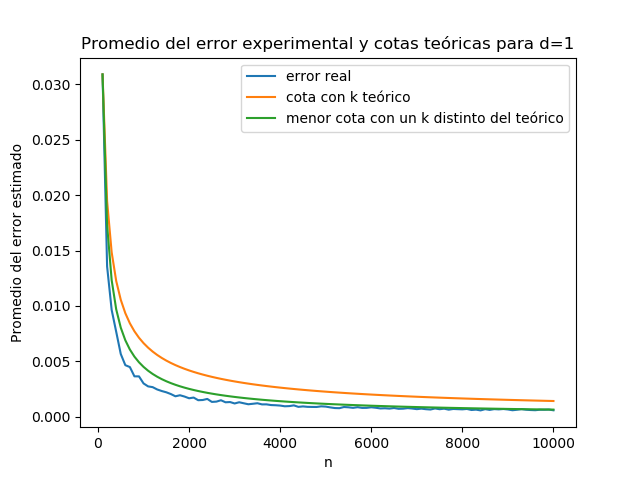
\includegraphics[width=\textwidth]{figuras_h=0.1/cotas-error-d=1}

\section{Primeros resultados: $h_n=0.1$}

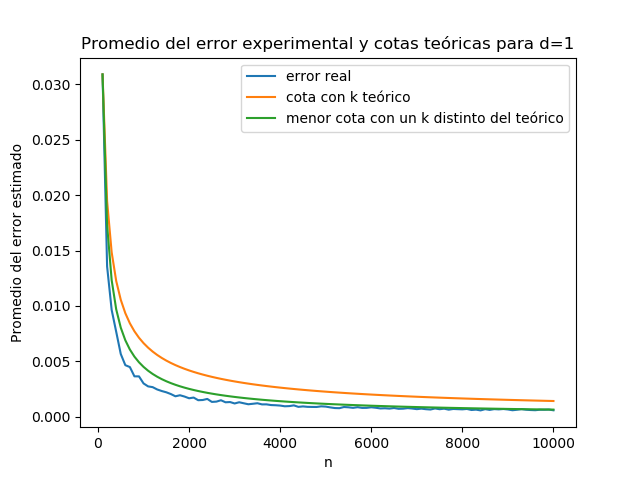
\includegraphics[width=0.5\textwidth]{figuras_h=0.1/cotas-error-d=1}
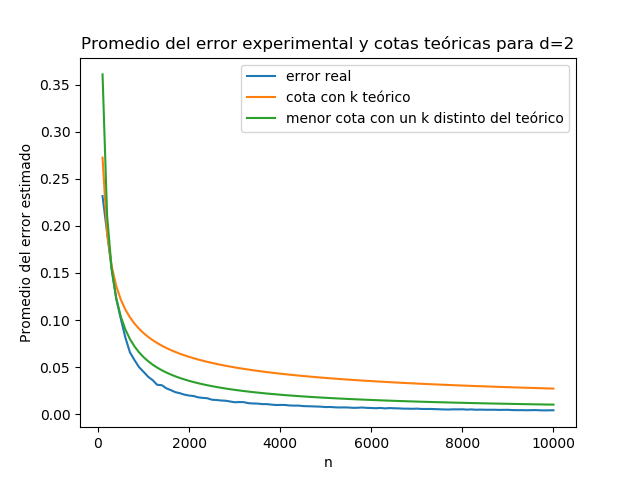
\includegraphics[width=0.5\textwidth]{figuras_h=0.1/cotas-error-d=2}
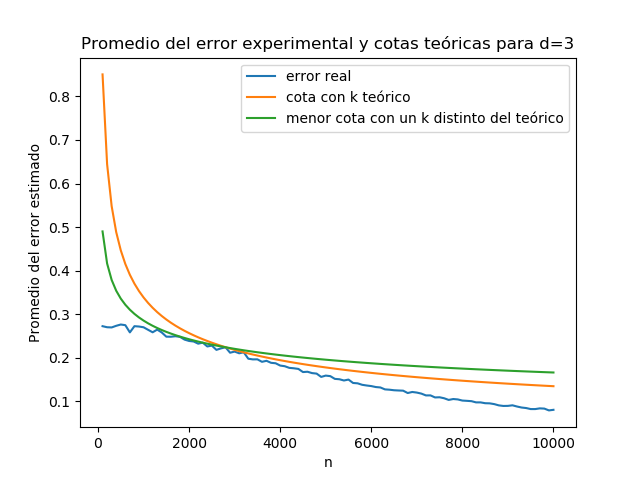
\includegraphics[width=0.5\textwidth]{figuras_h=0.1/cotas-error-d=3}
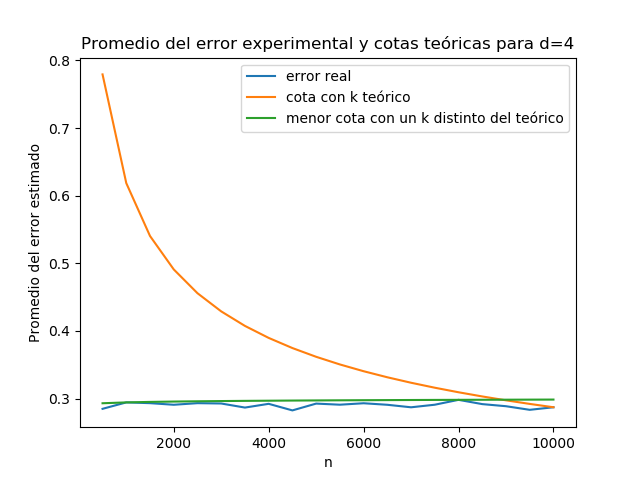
\includegraphics[width=0.5\textwidth]{figuras_h=0.1/cotas-error-d=4}
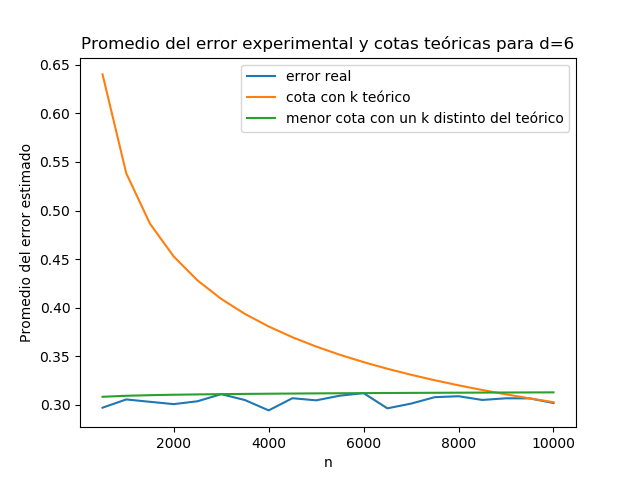
\includegraphics[width=0.5\textwidth]{figuras_h=0.1/cotas-error-d=6}
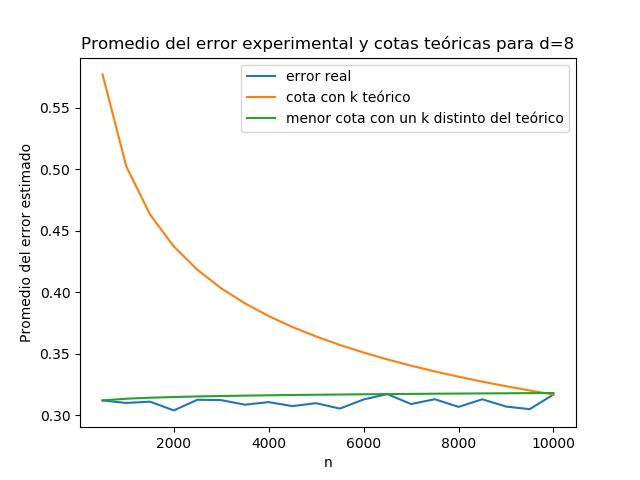
\includegraphics[width=0.5\textwidth]{figuras_h=0.1/cotas-error-d=8}
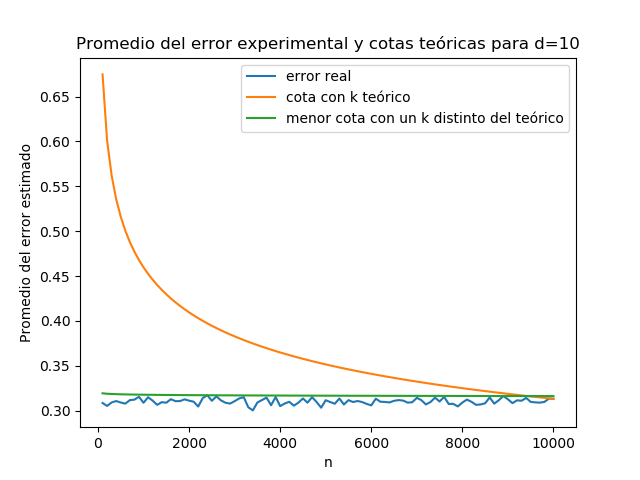
\includegraphics[width=0.5\textwidth]{figuras_h=0.1/cotas-error-d=10}
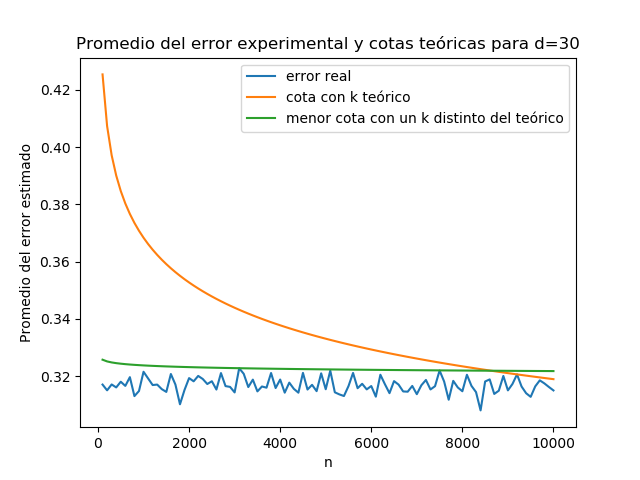
\includegraphics[width=0.5\textwidth]{figuras_h=0.1/cotas-error-d=30}

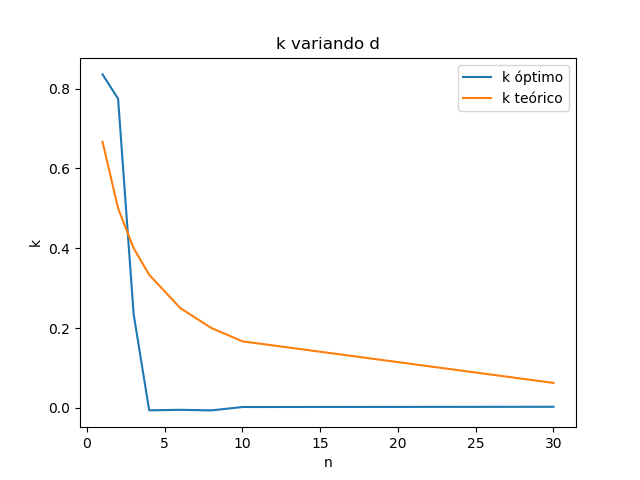
\includegraphics[width=\textwidth]{figuras_h=0.1/k-variando-d}

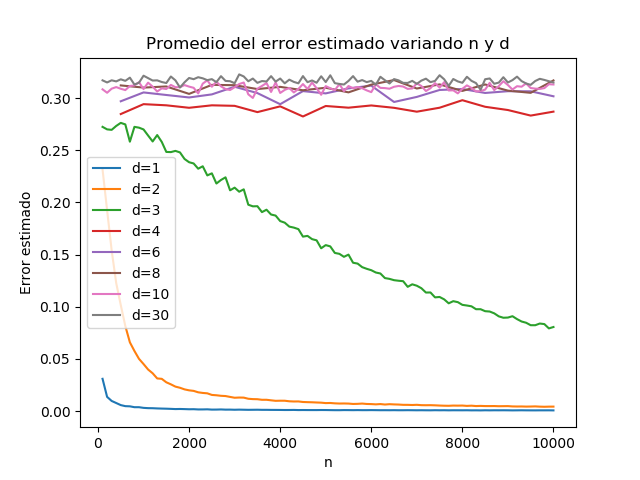
\includegraphics[width=\textwidth]{figuras_h=0.1/resultados-grales}


\section{Primeros resultados: $h_n=0.5$}

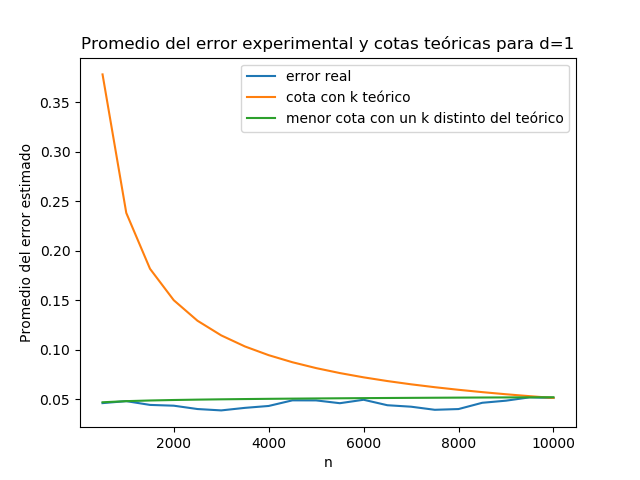
\includegraphics[width=0.5\textwidth]{figuras_h=0.5/cotas-error-d=1}
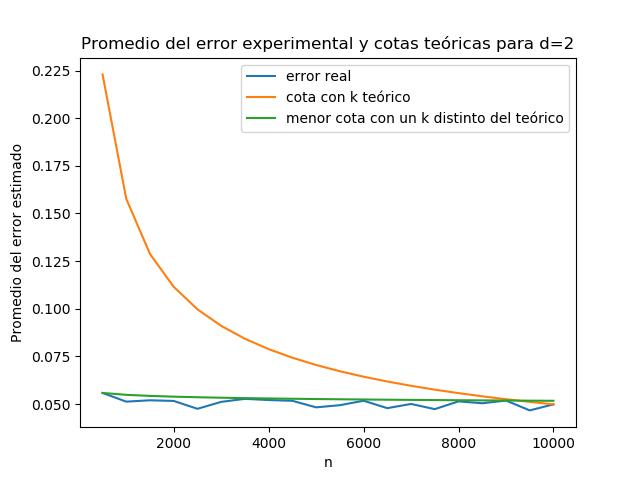
\includegraphics[width=0.5\textwidth]{figuras_h=0.5/cotas-error-d=2}
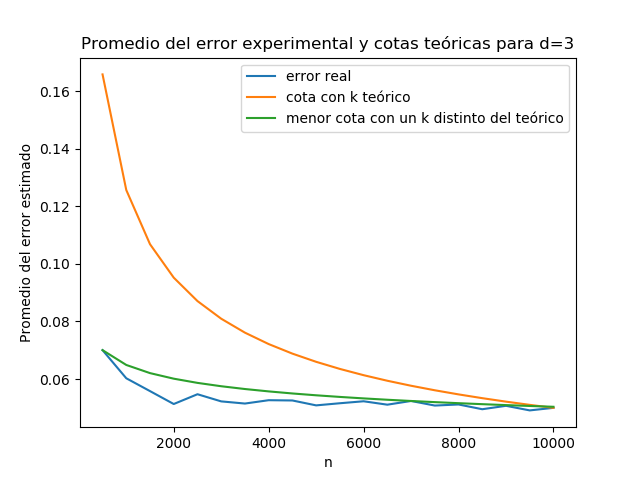
\includegraphics[width=0.5\textwidth]{figuras_h=0.5/cotas-error-d=3}
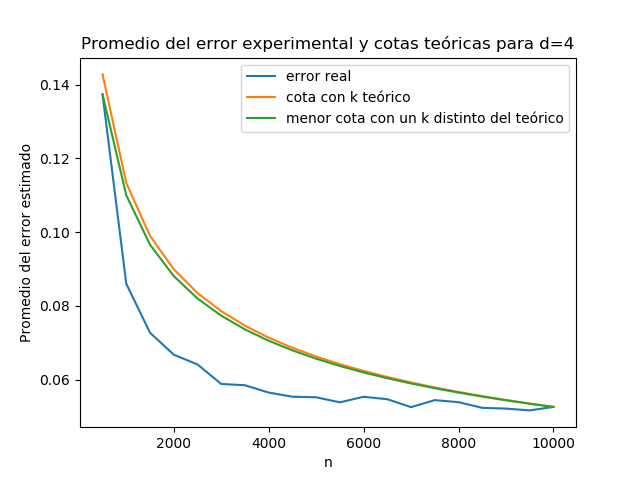
\includegraphics[width=0.5\textwidth]{figuras_h=0.5/cotas-error-d=4}
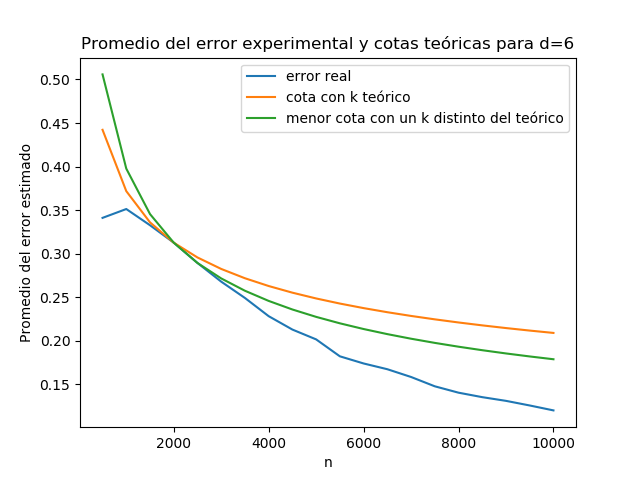
\includegraphics[width=0.5\textwidth]{figuras_h=0.5/cotas-error-d=6}
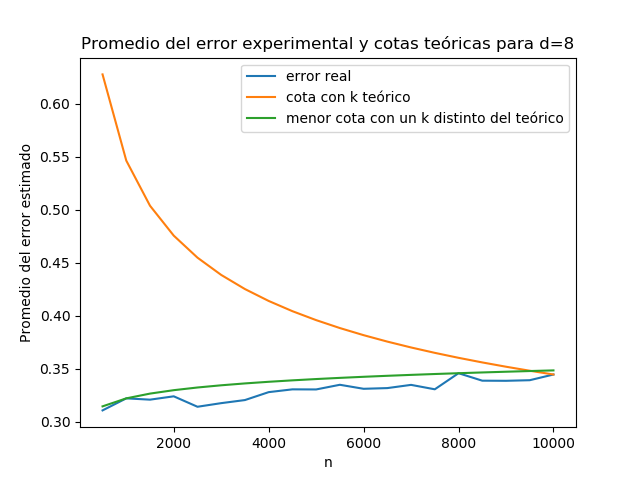
\includegraphics[width=0.5\textwidth]{figuras_h=0.5/cotas-error-d=8}
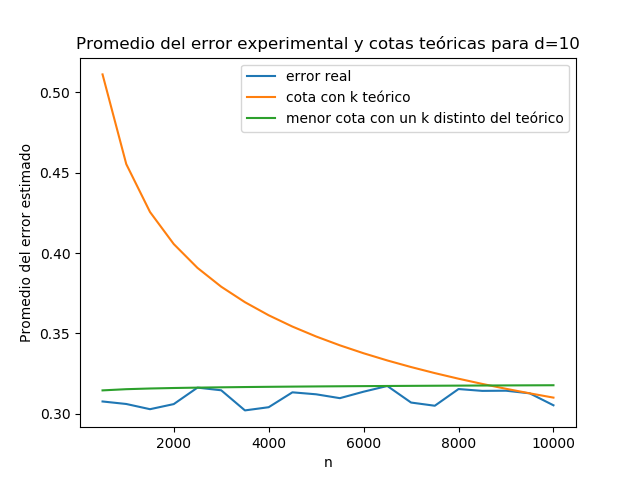
\includegraphics[width=0.5\textwidth]{figuras_h=0.5/cotas-error-d=10}

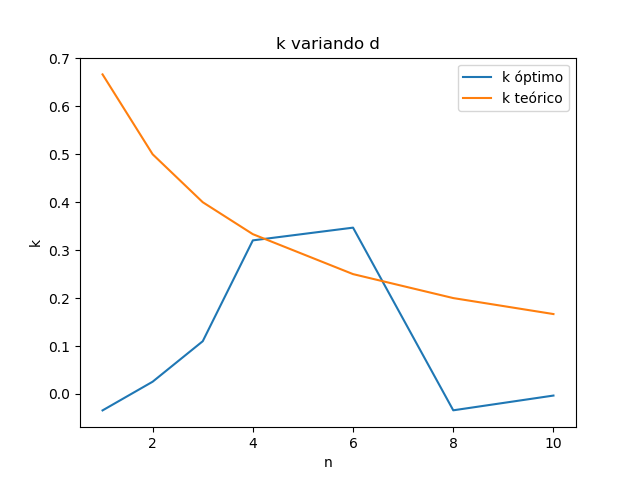
\includegraphics[width=\textwidth]{figuras_h=0.5/k-variando-d}

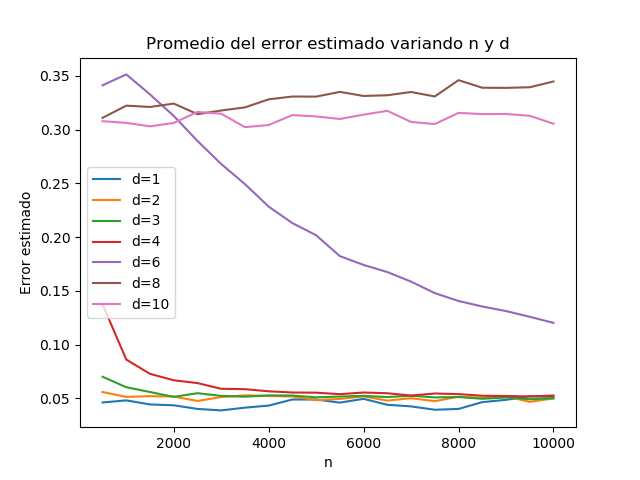
\includegraphics[width=\textwidth]{figuras_h=0.5/resultados-grales}

\section{Conclusiones para $h_n$ constante}
Para $h_n=0.1$ se obtuvieron resultados buenos (que verifican) para $d=1$, $d=2$ y $d=3$, pero para $d$ superiores no se logró la verificación. 

Esto es razonable cuando se tienen en cuenta las reglas usadas en la práctica "común" de machine learning: al aumentar la cantidad de dimensiones y no subsanar esto con más datos se tiene underfitting. 

En este caso en particular también es importante la maldición de la dimensionalidad: a medida que crece $d$, la cantidad de puntos a una distancia fija $h_n$ cae (en realidad, el mismísimo significado de la distancia es el que se pierde: todos los puntos tienden a estar a una distancia muy similar unos de otros).

Aunque las "reglas prácticas del machine learning" y la maldición de la dimensionalidad explican los resultados, estos contradicen al teorema que se busca corroborar empiricamente (es decir, la interpretación que se había hecho del mismo).

Con el objetivo de observar el comportamiento del algoritmo en dimensiones altas, se utilizó $h_n=0.5$ para realizar una nueva prueba.

Los resultados de esta prueba son muy importantes: para dimensiones "medianas"  ( $d=4$, $d=6$), con $h_n=0.5$ se logra lo que no se puede con $h_n=0.1$: se tiene una mejora gradual y se corrobora el teorema para $d=6$.

El problema es que fue ignorada la condición sobre $h_n$ que requiere la segunda conclusión del teorema:


$$
h_n = c' \Bigg( \dfrac{\sigma^2 + \mathop{sup}_{z\in S^{*}}|m(z)|^2 }{C^2} \Bigg)^{1/(d+2)} n^{\Big (-\dfrac{1}{d+2}\Big )}
$$

\section{Segunda estrategia}

Es imposible fijar 
$$
h_n = c' \Bigg( \dfrac{\sigma^2 + \mathop{sup}_{z\in S^{*}}|m(z)|^2 }{C^2} \Bigg)^{1/(d+2)} n^{\Big (-\dfrac{1}{d+2}\Big )}
$$
ya que para eso sería necesario conocer $c'$.

Entonces se intenta corroborar el teorema 5.1, que establece:

\begin{quotation}
\textbf{Theorem 5.1:} Assume that there are balls $S_{0,r}$ of radius $r$ and balls $S_{0,R}$
of radius $R$ centered at the origin ($0 < r\leq R$), and constant $b>0$ such that
$$
\mathds{1}\{x\in S_{0,R}\}\geq K(x) \geq b \mathds{1}\{x\in S_{0,r}\}
$$
(boxed kernel), and consider the kernel estimate $m_n$ if $h_n \rightarrow 0$ and $n h_n^d \rightarrow \infty$, then the kernel estimate is weakly universally consistent.
\end{quotation}

El kernel naive es un boxed kernel, por lo tanto, si se cumplen las condiciones sobre $h_n$ que establece este teorema, se obtiene la consistencia debil.

Así, se llevaron adelante dos pruebas: una con $h_n$ dependiendo de $n$ y $d$, y otra en la cual depende sólo de $d$. Así, para la primera, se usó $$ 0.8548 (n^{(-1/(4.054 \cdot d))}) $$, lo cual cumple las condiciones y además cumple que $h_n$ es aproximadamente $0.1$ cuando $d=1$ y $n=8000$, y aproximadamente $0.5$ cuando $d=4$ y $n=8000$. Para la segunda corrida de pruebas se utilizó $h_n=10^{-1/d}$, elegido con el mismo criterio.

\section{Resultados para $h_n$ variando con $d$ y $n$}

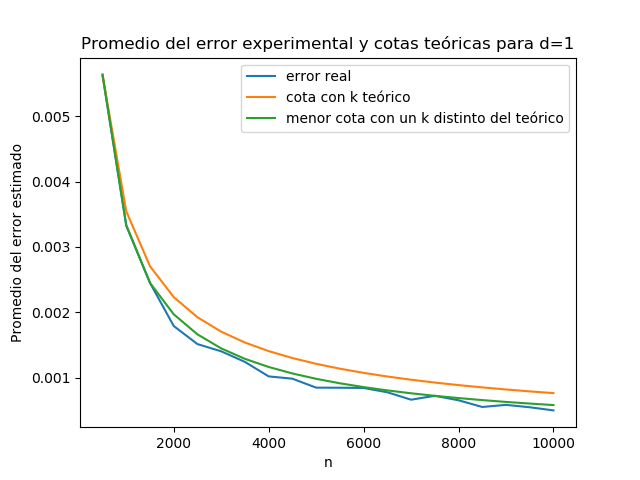
\includegraphics[width=0.5\textwidth]{figuras_h_dinamico/cotas-error-d=1}
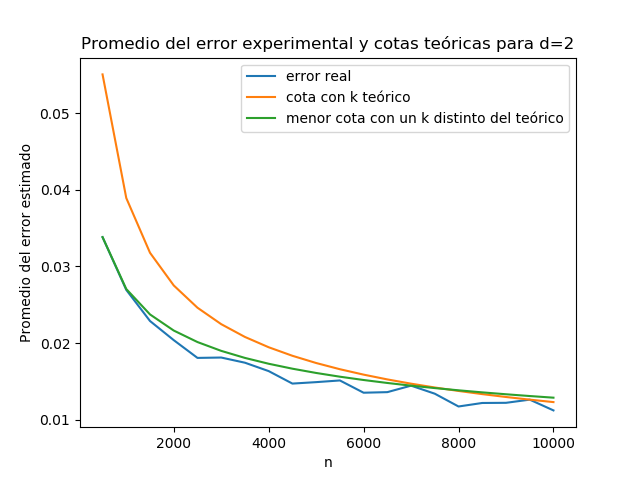
\includegraphics[width=0.5\textwidth]{figuras_h_dinamico/cotas-error-d=2}
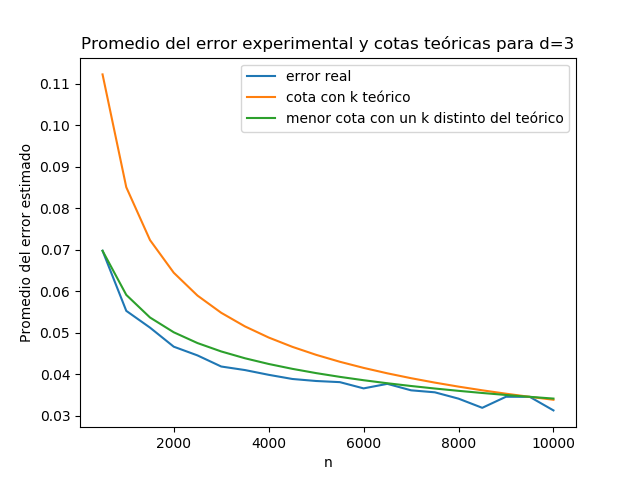
\includegraphics[width=0.5\textwidth]{figuras_h_dinamico/cotas-error-d=3}
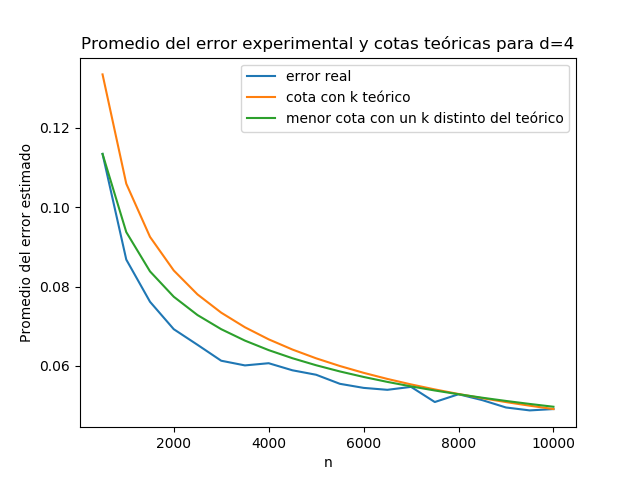
\includegraphics[width=0.5\textwidth]{figuras_h_dinamico/cotas-error-d=4}
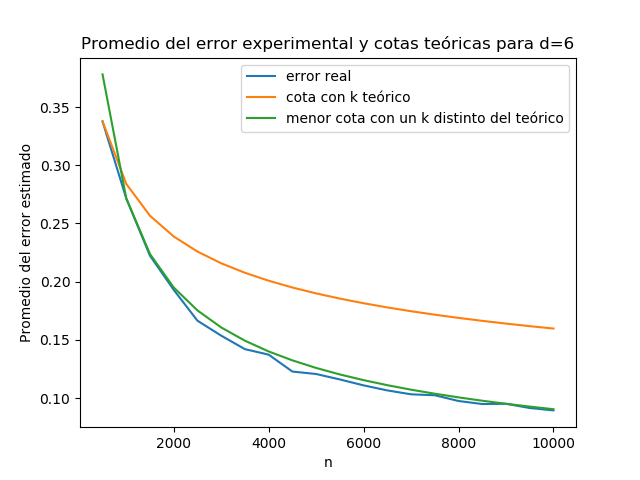
\includegraphics[width=0.5\textwidth]{figuras_h_dinamico/cotas-error-d=6}
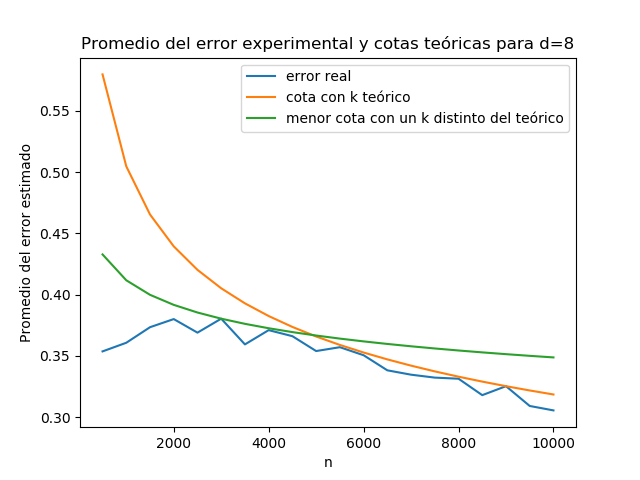
\includegraphics[width=0.5\textwidth]{figuras_h_dinamico/cotas-error-d=8}
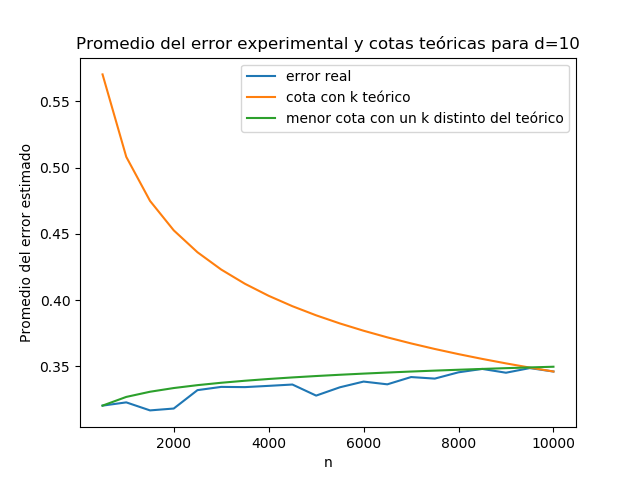
\includegraphics[width=0.5\textwidth]{figuras_h_dinamico/cotas-error-d=10}

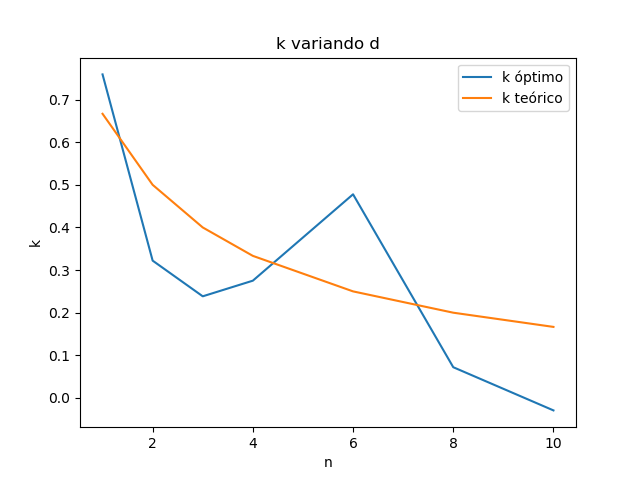
\includegraphics[width=\textwidth]{figuras_h_dinamico/k-variando-d}

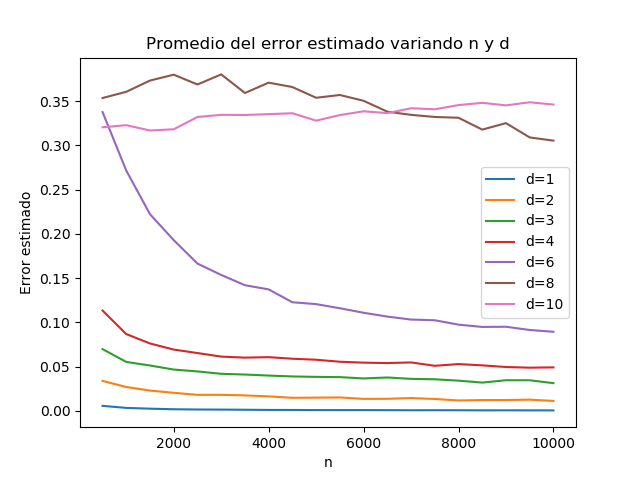
\includegraphics[width=\textwidth]{figuras_h_dinamico/resultados-grales}


\section{Resultados para $h_n$ variando sólo con $d$}

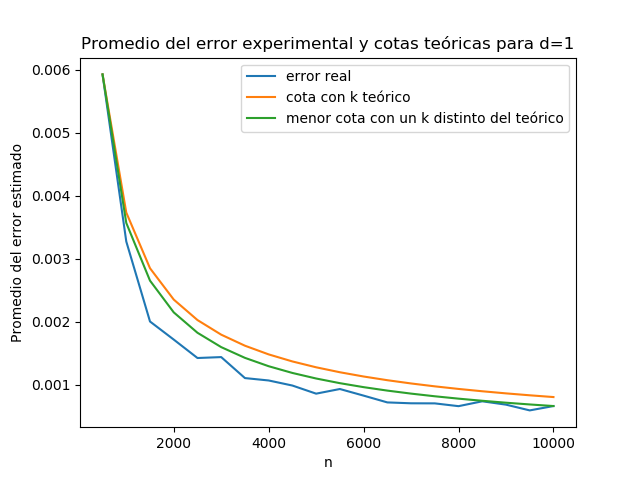
\includegraphics[width=0.5\textwidth]{figuras_h_semidinamico/cotas-error-d=1}
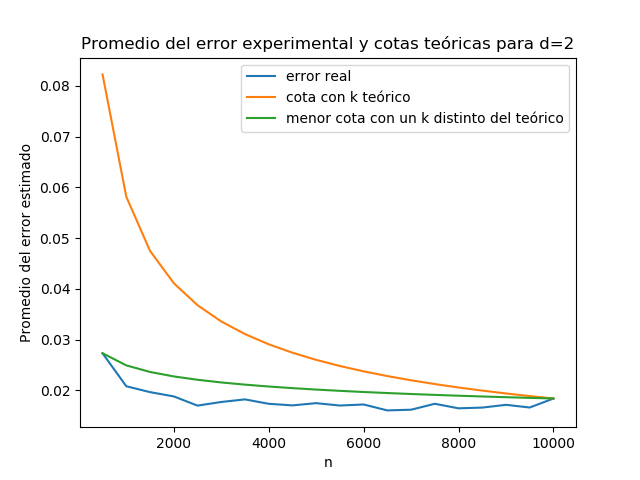
\includegraphics[width=0.5\textwidth]{figuras_h_semidinamico/cotas-error-d=2}
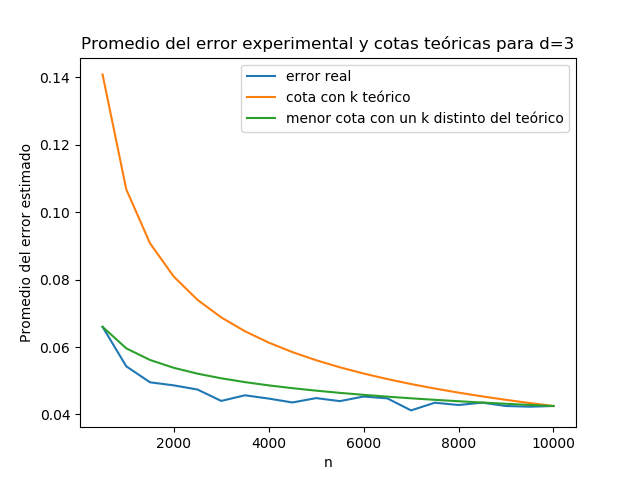
\includegraphics[width=0.5\textwidth]{figuras_h_semidinamico/cotas-error-d=3}
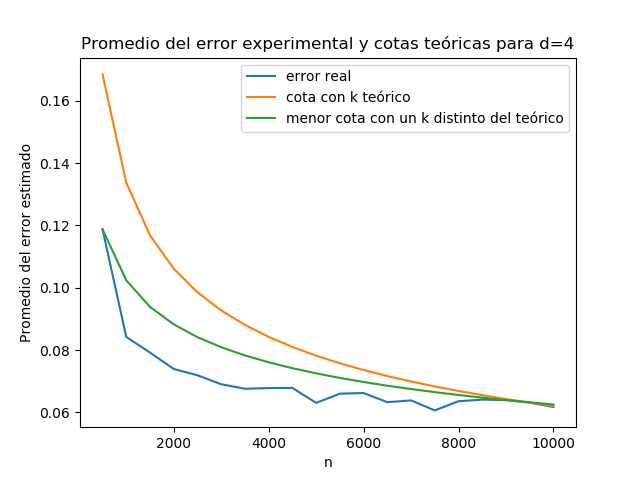
\includegraphics[width=0.5\textwidth]{figuras_h_semidinamico/cotas-error-d=4}
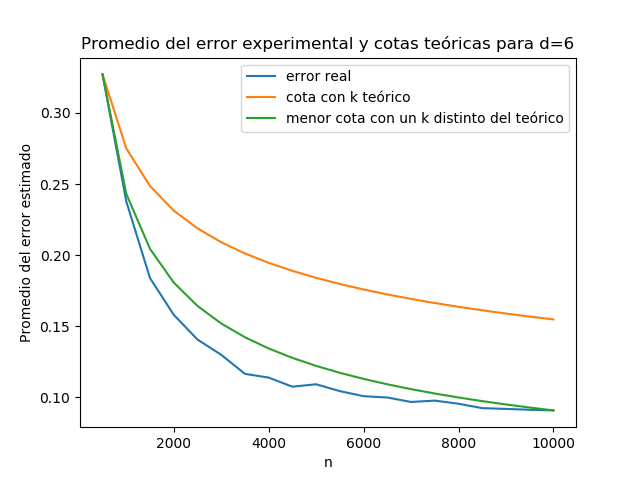
\includegraphics[width=0.5\textwidth]{figuras_h_semidinamico/cotas-error-d=6}
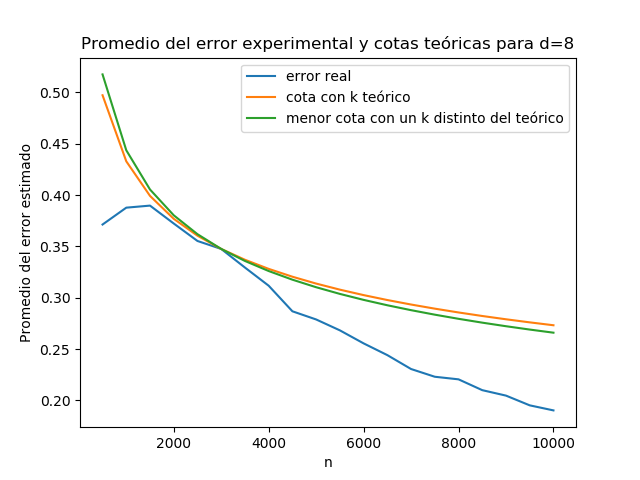
\includegraphics[width=0.5\textwidth]{figuras_h_semidinamico/cotas-error-d=8}
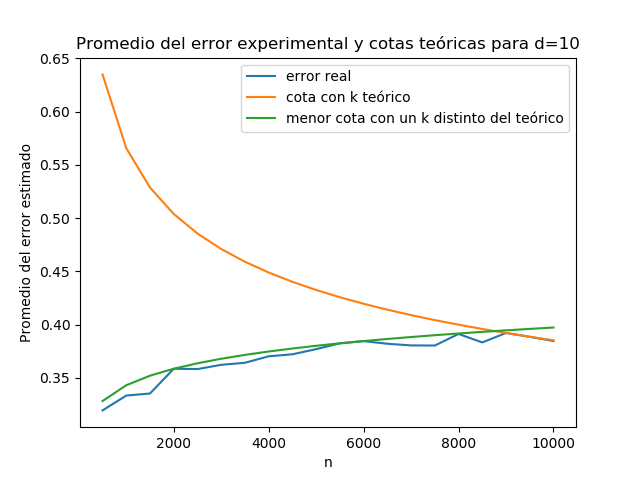
\includegraphics[width=0.5\textwidth]{figuras_h_semidinamico/cotas-error-d=10}

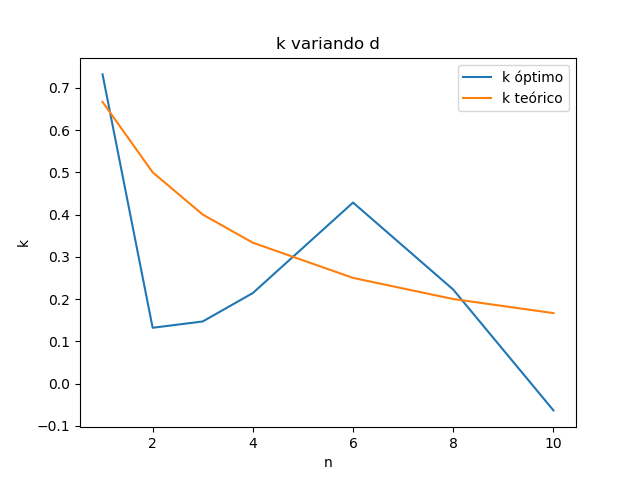
\includegraphics[width=\textwidth]{figuras_h_semidinamico/k-variando-d}

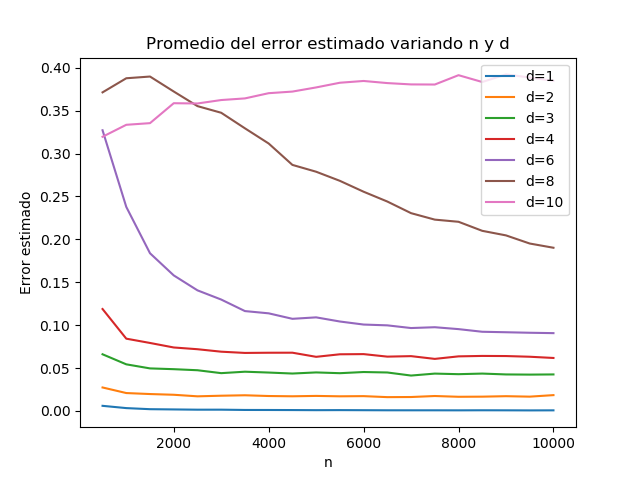
\includegraphics[width=\textwidth]{figuras_h_semidinamico/resultados-grales}

\section{Conclusiones para $h_n$ variable}

En caso de $h_n$ variable, se obtuvieron mejores resultados para todas las curvas: hubo aprendizaje para $d$ entre 1 y 6, lo cual era de esperar debido al criterio utilizado para elegir las constantes, discutido previamente; y también hubo aprendizaje para $d=8$, lo cual no se había observado para $h_n=0.1$ ni $h_n=0.5$. Esto es un indício fuerte para opinar que es posible corroborar el teorema 5.1.

El aprendizaje para $d=8$ es muy notorio para $h_n$ dependiente sólo de $d$, y menos notorio para $h_n$ dependiente de $n$, lo cual podría resultar contradictorio al teorema.

El hecho de que para $d=10$ no se dé el aprendizaje podría deberse a dos motivos:
\begin{enumerate}
  \item Las constantes elegidas para las funciones $h_n(n,d)$ y $h_n(d)$ son incorrectas.
  \item Las formas generales elegidas para $h_n(n,d)$ y $h_n(d)$ son incorrectas.
\end{enumerate}

Otra posibilidad es que el teorema sea imposible de corroborar en altas dimensiones debido a la maldición de la dimensionalidad: que el aprendizaje sea demasiado lento como para observarlo.



\end{document}
